\chapter{Methodology}
This chapter will look at the methodologies we used throughout the project regarding research, software development, client \& supervisor meetings, testing, project management and the tools used.

\section{Research Methodology}
For this project we chose a form of a Mixed Research Methodology which involves both Qualitative and Quantitative research.

\subsection{Qualitative}
Qualitative research is focused on exploring and finding out thoughts, ideas and opinions \cite{tesch2013qualitative}. This was suitable for our project at an early stage such as meeting the client initially. From this we gained invaluable insights into his goals, thoughts and ideas for the prototype. We also were given possible scenarios for the training application. An example was a ticket inspector (The player) would board the train and would be able to interact with any passenger to check if they had a ticket. From this scenario we conducted research into multiple areas such as chatbot technology, gamification and much more.

\subsection{Quantitative}
Quantitative research is less theoretical than qualitative research and is focused more on numerical results and statistics \cite{sukamolson2007fundamentals}. This research was used later in development when we had developed and deployed a test build. These builds were shown to the client and our supervisor. In return we collected the feedback, thoughts and ideas they had which was used to further make changes and achieve the initial outlined goals.

\section{Software Development Methodology}
We looked at several different approaches regarding software development methodologies, which included Waterfall and Agile methodologies. Waterfall is a sequential series steps or processes that must be completed before moving onto the following steps. These processes include (Requirements, Design, Implementation, Verification and Maintenance) \cite{cheatham1991object}. However, from initial research we decided it wouldn't suit our projects as it can exclude the client from the process, causing changes to be difficult to make and delay testing until the end of the project which would decrease software quality. Another methodology we looked at was Agile. Agile promotes continuous development, deployment and testing throughout the software development life cycle (SDLC) of the project to help increase productivity, software quality and decrease development time \cite{Cohen2003AgileSD}. We felt this would be most suitable to our project so we began to look at how Agile could be implemented to coincide with our initial goals.

\subsection{Agile - Extreme Programming}
The Agile methodology we have chosen for this project was Extreme Programming (XP). Extreme Programming is a form of Agile, which focuses on small development teams, quick iterative development cycles and a focus on test driven development. It is based on five values simplicity, communication, feedback, courage and respect. \cite[p.~4]{1335275620040101}. This iterative development cycle is outlined in figure~\ref{image:XP}

\begin{figure}[h!]
	\caption{Extreme Programming Life Cycle.}
	\label{image:XP}
	\centering
	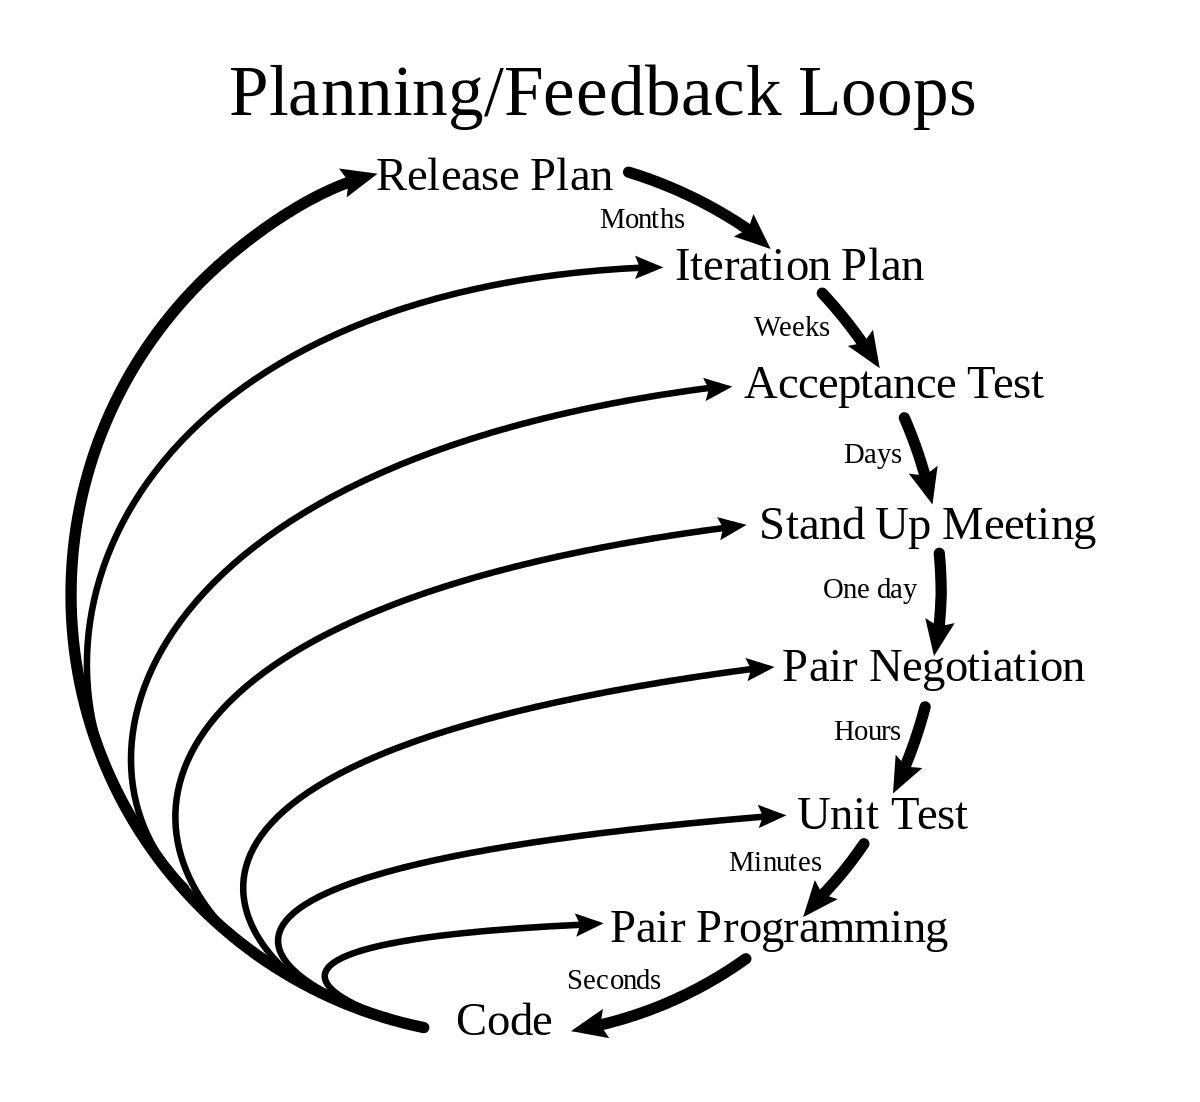
\includegraphics[width=0.65\textwidth]{Images/Extreme_Programming.png}
\end{figure}	

\subsubsection{Advantages}
\begin{itemize}
  \item Cuts down cost and time of software projects, due to a focus on timely delivery of final products and less time on cumbersome documentation. Also, problems are solved through group discussions and errors are spotted earlier with Peer reviews. Peer reviews involve two programmers sitting side by side working on a feature. This was helpful for us working in college as we could fix bugs quickly and efficiently.
  \item Feedback is constant, so changes can be made quickly and efficiently.
  \item Software is developed faster, due to constant testing and deployment.
  \item Simplicity is key, so code can be developed quickly to pass tests and meet goals, and then improved later.
  \item Works well with small and large teams, which would be suitable for our project.
\end{itemize}

\subsubsection{Disadvantages}
\begin{itemize}
  \item Not suitable for teams that are separated geographically.
  \item There can be a lack of defect documentation, so bugs can go unnoticed or not tested. However, we improved on this with GitHub issue tracking.
  \item The lack of full documentation can cause problems especially in larger projects or if team members leave/join midway.
\end{itemize}

As the advantages outweigh the disadvantages it was clear XP was the correct methodology to choose. Also, since it is more suited to the team size, workflow, project type and client.

\section{Meetings}
Initially we met with both our supervisor and our client. In this meeting we discussed initial goals, thoughts and ideas for the project (Qualitative Research). We also outlined the minimum requirements for the prototype which are described in the introduction chapter. Each week we would then meet our supervisor to discuss the following.

\begin{itemize}
  \item Our progress from the last meeting.
  \item Feedback on our progress.
  \item Our next steps and planning.
  \item Answer any questions from our client or supervisor. 
\end{itemize}

The frequency of meetings fitted well with XP perfectly as we could make any changes that arose from the meeting, then test and deploy the project again for the following week to show our supervisor.

\section{Testing}
Throughout the project we incorporated multiple testing methodologies such as Functional and Non-functional testing. More information on how these methodologies were implemented can found in the System Evaluation chapter.

\subsection{Functional Testing}
Functional testing focuses the functional aspects of a system such as unit, integration and system testing.

\subsubsection{Unit testing}
Unit testing is the first form of testing to be completed and is usually undertaken by the developer themselves. It involves testing a class level, E.g. testing functions in a class if they behave correctly and don't produce errors \cite{5380492}. We implemented tests using NUnit framework to test basic functions of the Unity game. We also used pytest to run unit tests on the server. To test HTTP methods from the application to the server we used Postman to check the packets and debug errors.

\subsubsection{Integration testing}
Integration testing involves testing the system to insure it still works when adding new features, so it doesn't break other areas of the system \cite{5380492}. We implemented integration by testing for all aspects of the system to see if they still worked correctly on all iterative builds. This was especially useful when adding Oculus VR support as it caused multiple errors with the Azure speech services.

\subsubsection{System testing}
System testing is a black box testing methodology completed after integration testing to ensure the system meets the requirements \cite{1028373}. We implemented system testing by ensuring the application met the initial requirements outlined by the client in the Introduction Chapter.

\subsection{Non-functional Testing}
Non-functional testing focuses on the non-functional aspects of a system such as performance, usability and compatibility.

\subsubsection{Performance testing}
Compatibility testing is a measure of how the system performs under pressure, or heavy load \cite{1028373}. We tested the system with a high number of requests to the server to ensure it didn't buckle under load. We also recorded the time requests took to process which was largely dependant on internet speed. This was one of the technical limitations of the project.

\subsubsection{Security testing}
Security testing involves testing how secure the system is against unauthorized attacks \cite{1028373}. We implemented security measures regarding the server, deployment and database access.

\subsubsection{Usability testing}
Usability testing involves measuring the ease of use from and end user’s perspective \cite{5380492}. This was vital to our game as it's a training experience, so we spent a lot of time working on improving usability of all controls, menus and game play. We conducted user tests with multiple users and our supervisor to collect data.

\subsubsection{Compatibility testing}
Compatibility testing is a measure of how well a system works in different environments (Browsers, devices etc.) \cite{5380492}. This was essential as we were developing the application to work on Android, Windows, and Oculus Quest VR.

\section{Project Management}
We have used Git with GitHub to track our changes, log error and work effectively using our chosen Agile methodology. Git is an open source and free version control system which allows small or large projects to be stored and accessed efficiently \cite{github}. Features include commits, branching, staging and workflows. GitHub allows a project to be stored remotely and for multiple people to work together seamlessly. 
\par
\medskip

Using GitHub and Git allowed us to work simultaneously on the project to increase our productivity. We also used the inbuilt features on GitHub such as issue tracking. If an issue occurred or a bug was found during testing, we would make a GitHub issue, and log all our commits using the issue id. This would track our progress in fixing it and help us keep an account of the work undertaken.

\section{Development Tools}
For this project we used a multitude of tools to develop each section. The main tool that was used was the Unity Editor and Visual Studio. The Unity version used was 2019.2.6f1 which includes all the new features and provided support for the Azure Speech Services used. All the Unity script were written using Visual Studio in C\#. Visual Studio was useful as it included the required packages and IntelliSense for creating Unity scripts. The flask server was developed using Visual Studio code and was initially deployed to an AWS EC2 (Amazon Elastic Computer Cloud). Later it was deployed and modified using Heroku, and then finally PythonAnywhere.
